\subsection{Line-line picking}
\label{sec:line_line}

In the simplest case, two points are chosen IID uniformly from a line
of length $L$. 

Figure~\ref{fig:hyperball_pdf} shows the PDF for the problem for the
case $L=1$.

\begin{figure}[tbp]
  \begin{center}
    \subfloat[\label{fig:hyperball_pdf}PDF of length 1 line showing
    exact and simulated values.]{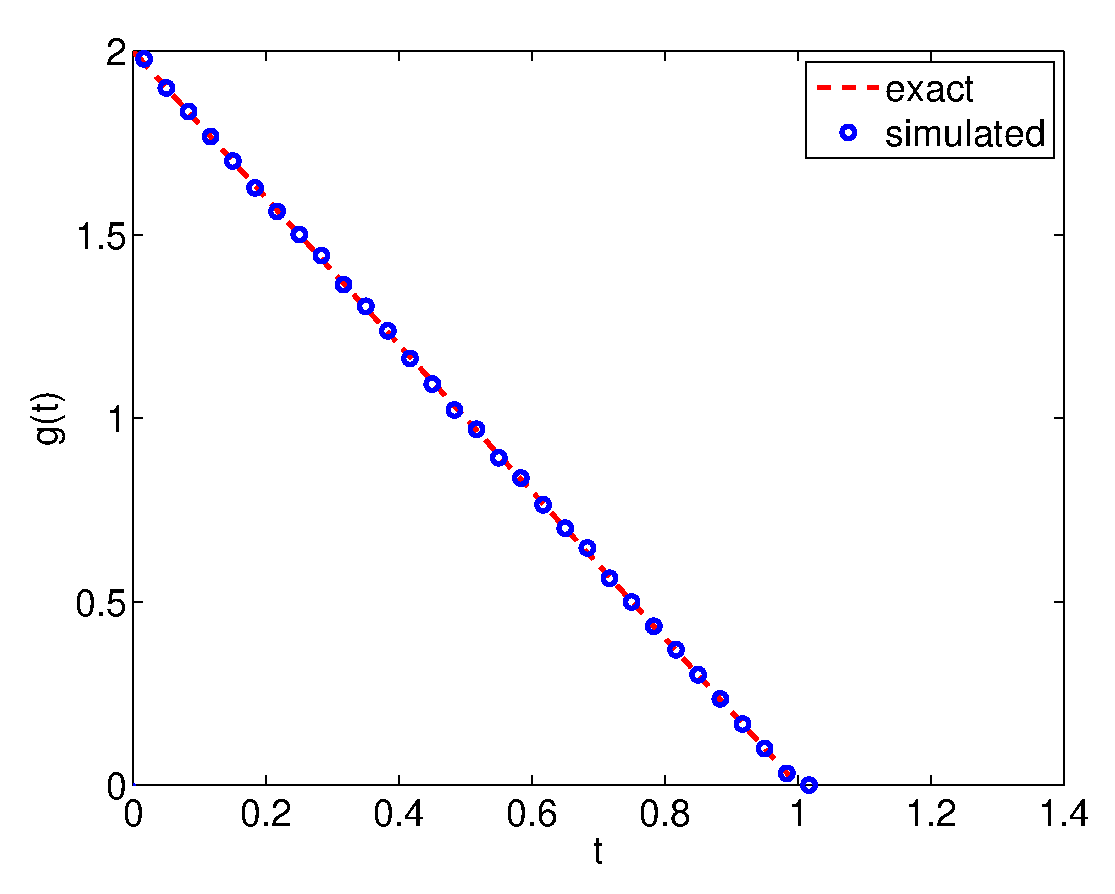
\includegraphics[width=0.48\columnwidth]{../Matlab/Plots/LinePicking_test_sim_line.eps}}
    \caption{The line-line picking problem ($L=1$).}
  \end{center} 
\vspace{-4mm}
\end{figure}

\subsubsection{PDF}

The probability density function of distances between two (uniformly)
randomly chosen points on the unit line is given in
\cite{weisstein:_line_line_picking,b.ghosh51:_random_rect}, as
\begin{equation}
  \label{eq:line_line}
  g^{\rm line}(t) = 2(1-t),
\end{equation}
or for a line of length $L$ as
\begin{equation}
  \label{eq:line_lineL}
  g^{\rm line}_L(t) = \frac{2}{L} \left( 1-\frac{t}{L} \right).
\end{equation}

This also arises as the limit as $a \rightarrow 0$ for the PDF for the
rectangle \eqref{eqn:rectangle}.

\subsubsection{CDF}


\subsubsection{Moments}




